%%%%%%%%%%%%%%%%%%%%%%%%%%%%%%%%%%%%%%%%%
% Beamer Presentation
% LaTeX Template
% Version 1.0 (10/11/12)
%
% This template has been downloaded from:
% http://www.LaTeXTemplates.com
%
% License:
% CC BY-NC-SA 3.0 (http://creativecommons.org/licenses/by-nc-sa/3.0/)
%
%%%%%%%%%%%%%%%%%%%%%%%%%%%%%%%%%%%%%%%%%

%----------------------------------------------------------------------------------------
%	PACKAGES AND THEMES
%----------------------------------------------------------------------------------------

\documentclass{beamer}

\mode<presentation> {

% The Beamer class comes with a number of default slide themes
% which change the colors and layouts of slides. Below this is a list
% of all the themes, uncomment each in turn to see what they look like.

%\usetheme{default}
%\usetheme{AnnArbor}
%\usetheme{Antibes}
%\usetheme{Bergen}
%\usetheme{Berkeley}
%\usetheme{Berlin}
%\usetheme{Boadilla}
%\usetheme{CambridgeUS}
%\usetheme{Copenhagen}
\usetheme{Darmstadt}
%\usetheme{Dresden}
%\usetheme{Frankfurt}
%\usetheme{Goettingen}
%\usetheme{Hannover}
%\usetheme{Ilmenau}
%\usetheme{JuanLesPins}
%\usetheme{Luebeck}
%\usetheme{Madrid}
%*\usetheme{Malmoe}
%\usetheme{Marburg}
%\usetheme{Montpellier}
%\usetheme{PaloAlto}
%\usetheme{Pittsburgh}
%\usetheme{Rochester}
%\usetheme{Singapore}
%\usetheme{Szeged}
%\usetheme{Warsaw}

% As well as themes, the Beamer class has a number of color themes
% for any slide theme. Uncomment each of these in turn to see how it
% changes the colors of your current slide theme.

%\usecolortheme{albatross}
%\usecolortheme{beaver}
%\usecolortheme{beetle}
%\usecolortheme{crane}
%\usecolortheme{dolphin}
%\usecolortheme{dove}
%\usecolortheme{fly}
%\usecolortheme{lily}
\usecolortheme{orchid}
%\usecolortheme{rose}
%\usecolortheme{seagull}
%\usecolortheme{seahorse}
%\usecolortheme{whale}
%\usecolortheme{wolverine}

%\setbeamertemplate{footline} % To remove the footer line in all slides uncomment this line
%\setbeamertemplate{footline}[page number] % To replace the footer line in all slides with a simple slide count uncomment this line

%\setbeamertemplate{navigation symbols}{} % To remove the navigation symbols from the bottom of all slides uncomment this line
}


\usepackage{graphicx} % Allows including images
\usepackage{booktabs} % Allows the use of \toprule, \midrule and \bottomrule in tables
\usepackage{xspace}
\usepackage{caption}
\usepackage{subfigure}
\usepackage[english,brazil]{babel}
\usepackage[utf8]{inputenc}

%Renomeia o nome padrao das figuras.
\renewcommand{\figurename}{Figura}
\renewcommand{\tablename}{Tabela}
%----------------------------------------------------------------------------------------
%	TITLE PAGE
%----------------------------------------------------------------------------------------

\title[Computação Gráfica]{Visão Computacional e Computação Gráfica} % The short title appears at the bottom of every slide, the full title is only on the title page

\author{Uéliton Freitas} % Your name
\institute[UFMS] % Your institution as it will appear on the bottom of every slide, may be shorthand to save space
{
Universidade Católica Don Bosco - UCDB \\ % Your institution for the title page
\medskip
\textit{freitas.ueliton@gmail.com} % Your email address
}
\date{\today} % Date, can be changed to a custom date


\begin{document}

\begin{frame}
\titlepage % Print the title page as the first slide
\end{frame}

\begin{frame}
\frametitle{Sumário} % Table of contents slide, comment this block out to remove it
\tableofcontents % Throughout your presentation, if you choose to use \section{} and \subsection{} commands, these will automatically be printed on this slide as an overview of your presentation
\end{frame}




%----------------------------------------------------------------------------------------
%	PRESENTATION SLIDES
%----------------------------------------------------------------------------------------

%------------------------------------------------
\section{Formação de Imagens} 
%------------------------------------------------

%\section{Speeded-Up Robust Features - SURF} % A subsection can be created just before a set of slides with a common theme to further break down your presentation into chunks
%\section{Baf Of Features and Colors}

%\section{Refer\^encias}
%%%%%%%%%%%%%%%%%%%%%%%%%%%%%%%%%%%%%%%%%%%%%%%%%%%%%%%%%%%%%%%%%%%%%%%%%%%%%%%%%%%%%%%%%%

%\section{Refer\^encias}


%%%%%%%%%%%%%%%%%%%%%%%%%%%%%%%%%%%%%%%%%%%%%%%%%%%%%%%%%%%%%%%%%%%%%%%%%%%%%%%%%%%%%%%%%%
\begin{frame}
\frametitle{Formação de Imagens}

	\begin{figure}[htb!]
  		\centering
      		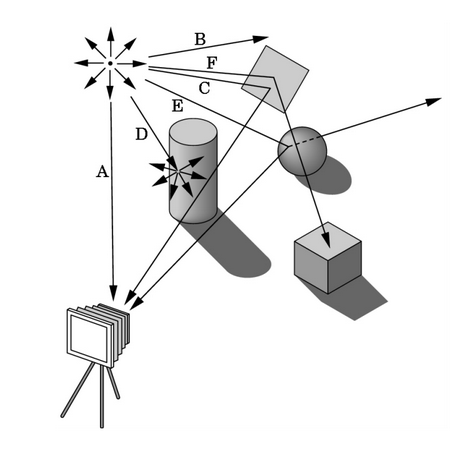
\includegraphics[width=0.6\textwidth]{Figures/raytracing}
      		\caption{Ray Tracing.}
  		\label{iep}
	\end{figure}


\end{frame}

%%%%%%%%%%%%%%%%%%%%%%%%%%%%%%%%%%%%%%%%%%%%%%%%%%%%%%%%%%%%%%%%%%%%%%%%%%%%%%%%%%%%%%%%%%
\begin{frame}
\frametitle{Formação de Imagens}

	\begin{block}{Como uma imagem é Formada?}
		\begin{itemize}
			\item Deve haver ajustes quanto a distância do objeto.
		\end{itemize}
	\end{block}
	\begin{figure}[htb!]
  		\centering
      		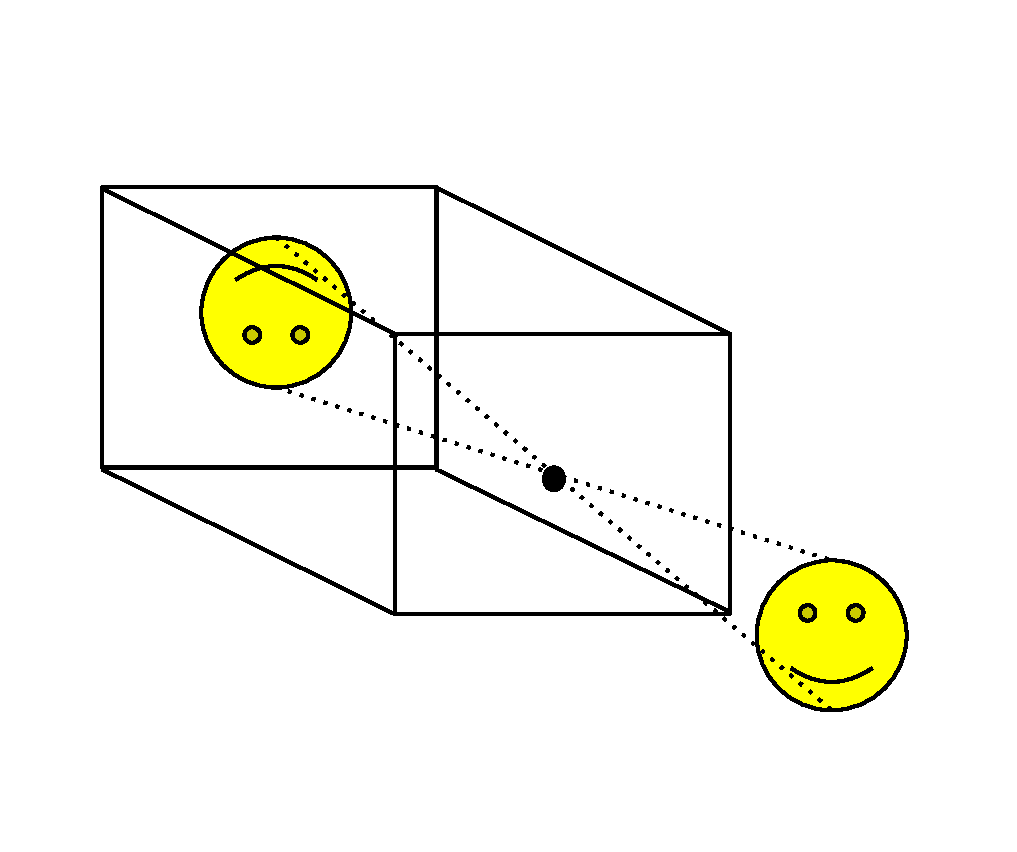
\includegraphics[width=0.6\textwidth]{Figures/pinHoleCam}
      		\caption{Pin Hole Cam.}
  		\label{iep}
	\end{figure}


\end{frame}



%%%%%%%%%%%%%%%%%%%%%%%%%%%%%%%%%%%%%%%%%%%%%%%%%%%%%%%%%%%%%%%%%%%%%%%%%%%%%%%%%%%%%%%%%%

\begin{frame}
\frametitle{Formação de Imagens}

	\begin{block}{Qual o tamanho do pin hole?}
		\begin{itemize}
			\item Se pequeno há Difração da luz.
			\item Caso seja grande o objeto fica borrado.
		\end{itemize}
	\end{block}
	
	\begin{figure}[htb!]
  		\centering
      		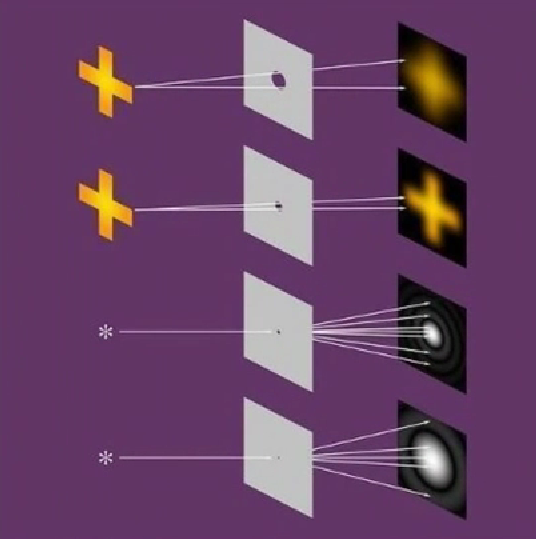
\includegraphics[width=0.5\textwidth]{Figures/pinHole}
      		\caption{Tamanho do Pin Hole.}
  		\label{iep}
	\end{figure}

\end{frame}


%%%%%%%%%%%%%%%%%%%%%%%%%%%%%%%%%%%%%%%%%%%%%%%%%%%%%%%%%%%%%%%%%%%%%%%%%%%%%%%%%%%%%%%%%%
\begin{frame}
\frametitle{Formação de Imagens}

	\begin{block}{Como resolver o problema do tamanho do pin hole?}
		\begin{itemize}
			\item As lentes substituem o pin hole.
			\item Com a curvatura correta, há maior incidência de raios de luz na formação das imagens.
			\item Contudo há problemas com o foco. É necessário ajusta-lo para a formação da imagem.
			\item Os raios não possuem a mesma intensidade em toda a lente.
		\end{itemize}
	\end{block}
	
	\begin{figure}[htb!]
  		\centering
      		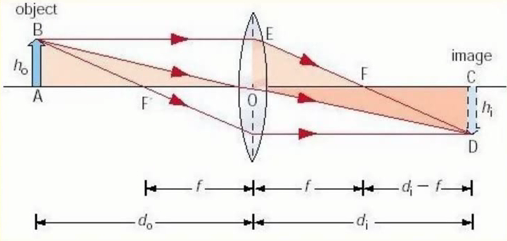
\includegraphics[width=0.5\textwidth]{Figures/lente}
  		\label{iep}
	\end{figure}

\end{frame}

%%%%%%%%%%%%%%%%%%%%%%%%%%%%%%%%%%%%%%%%%%%%%%%%%%%%%%%%%%%%%%%%%%%%%%%%%%%%%%%%%%%%%%%%%%
\begin{frame}
\frametitle{Formação de Imagens}

	\begin{block}{O olho humano.}
		\begin{itemize}
			\item Retina = CCD/Filme da câmera.
			\item Pupila + Iris = Diafragma (Orifício por onde a luz passa).
			\item Cristalino + Córnea = Lentes.
			\item Pálpebras = Obturador.
		\end{itemize}
	\end{block}
	
	\begin{figure}[htb!]
  		\centering
      		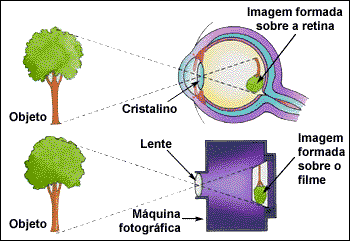
\includegraphics[width=0.5\textwidth]{Figures/olho_humano}
  		\label{iep}
	\end{figure}

\end{frame}

%%%%%%%%%%%%%%%%%%%%%%%%%%%%%%%%%%%%%%%%%%%%%%%%%%%%%%%%%%%%%%%%%%%%%%%%%%%%%%%%%%%%%%%%%%
\begin{frame}
\frametitle{Formação de Imagens}

	\begin{block}{Câmera Digital}
		\begin{itemize}
			\item O CCD que ``transforma'' a luz em dados interpretáveis.
			\item É gerada uma matriz de números que representa a imagem.
		\end{itemize}
	\end{block}
	
	\begin{figure}[htb!]
  		\centering
      		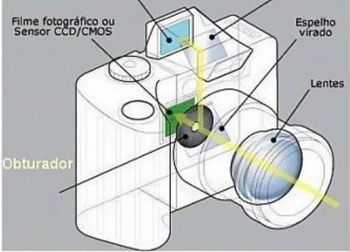
\includegraphics[width=0.5\textwidth]{Figures/cameraDigital}
  		\label{iep}
	\end{figure}

\end{frame}


%%%%%%%%%%%%%%%%%%%%%%%%%%%%%%%%%%%%%%%%%%%%%%%%%%%%%%%%%%%%%%%%%%%%%%%%%%%%%%%%%%%%%%%%%%
\begin{frame}
\frametitle{Formação de Imagens}

	\begin{block}{Câmera Digital}
		\begin{itemize}
			\item O CCD que ``transforma'' a luz em dados interpretáveis.
			\item É gerada uma matriz de números que representa a imagem.
		\end{itemize}
	\end{block}


\begin{table}[thb]
\caption{\label{}Representação de um CCD.}
\scriptsize
\centering
\begin{tabular}{|c|c|c|c|c|c|c|c|}
\hline 
222 & 187 & 23 & ... & 98 & 98 & 3 & 0	 \\ 
\hline 
231 & 34 & 67 & ... & 12 & 98 & 12 & 9	 \\ 
\hline 
211 & 32 & 14 & ... & 32 & 98 & 232 & 17	 \\ 
\hline 
12 & 34 & 123 & ... & 1 & 98 & 134 & 12	 \\ 
\hline 
... & ... & ... & ... & ... & ... & ... & ...	 \\  
\hline 
143 & 34 & 155 & ... & 32 & 98 & 132 & 15	 \\  
\hline 
163 & 34 & 164 & ... & 56 & 98 & 231 & 87	 \\ 
\hline 
153 & 34 & 123 & ... & 175 & 98 & 143 & 73	 \\ 
\hline 
174 & 125 & 253 & ... & 175 & 98 & 178 & 22	 \\ 
\hline 
\end{tabular} 
\end{table}
\end{frame}


%%%%%%%%%%%%%%%%%%%%%%%%%%%%%%%%%%%%%%%%%%%%%%%%%%%%%%%%%%%%%%%%%%%%%%%%%%%%%%%%%%%%%%%%%%

\begin{frame}
\frametitle{Visão Computacional x Computação Gráfica}

 \begin{columns}
    \begin{column}{0.5\textwidth}
      	\begin{block}{Visão Computacional}
			\begin{itemize}
				\item Extrair modelos de uma imagem.
				\item Utiliza algoritmos de aprendizado automático.
				\item Utiliza algoritmos de aprendiz
			\end{itemize}
		\end{block}
    \end{column}
    \begin{column}{0.5\textwidth}
      	\begin{block}{Computação Gráfica}
			\begin{itemize}
				\item Utilizar modelos matemáticos.
				\item Formam imagens a partir dos modelos.
				\item Tem foco em algoritmos de renderização, entre outros.
			\end{itemize}
		\end{block}
    \end{column}
    \end{columns}
	


\end{frame}

%%%%%%%%%%%%%%%%%%%%%%%%%%%%%%%%%%%%%%%%%%%%%%%%%%%%%%%%%%%%%%%%%%%%%%%%%%%%%%%%%%%%%%%%%%
\section{Visão Computacional}
%%%%%%%%%%%%%%%%%%%%%%%%%%%%%%%%%%%%%%%%%%%%%%%%%%%%%%%%%%%%%%%%%%%%%%%%%%%%%%%%%%%%%%%%%%

\begin{frame}
\frametitle{Visão Computacional}
	\begin{block}{Características da Visão Computacional}
	
		\begin{itemize}
			\item<1-> Adiciona ``sentido'' a visão da máquina.
			\item<2-> Problema complexo que envolve ``inteligência''.
			\item<3-> Inicia-se pela análise de uma imagem. 
			\item<4-> Utiliza técnicas para extrair atributos das imagens.
			\item<5-> Implementa no computador tarefas que requerem habilidades visuais. 
			\item<6-> Utiliza \textit{Machine Learning} para analisar interpretar as imagens.
		\end{itemize}
	\end{block}
\end{frame}


%%%%%%%%%%%%%%%%%%%%%%%%%%%%%%%%%%%%%%%%%%%%%%%%%%%%%%%%%%%%%%%%%%%%%%%%%%%%%%%%%%%%%%%%%%

\begin{frame}
\frametitle{Visão Computacional}
	\begin{block}{Exemplo de Visão Computacional}
		Exemplo de detecção de digitais.
	\end{block}
	\begin{figure}[!h]
		\begin{center}
			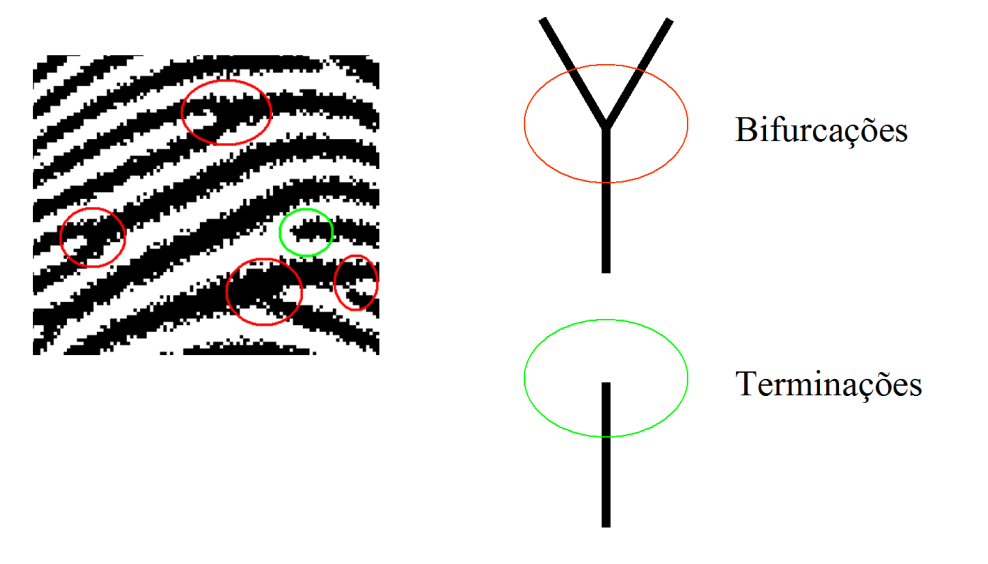
\includegraphics[width=0.9\textwidth]{Figures/bifdigitais}
		\end{center}
		
	\end{figure}
	
\end{frame}


%%%%%%%%%%%%%%%%%%%%%%%%%%%%%%%%%%%%%%%%%%%%%%%%%%%%%%%%%%%%%%%%%%%%%%%%%%%%%%%%%%%%%%%%%%

\begin{frame}
\frametitle{Visão Computacional}

	\begin{figure}[!h]
		\begin{center}
			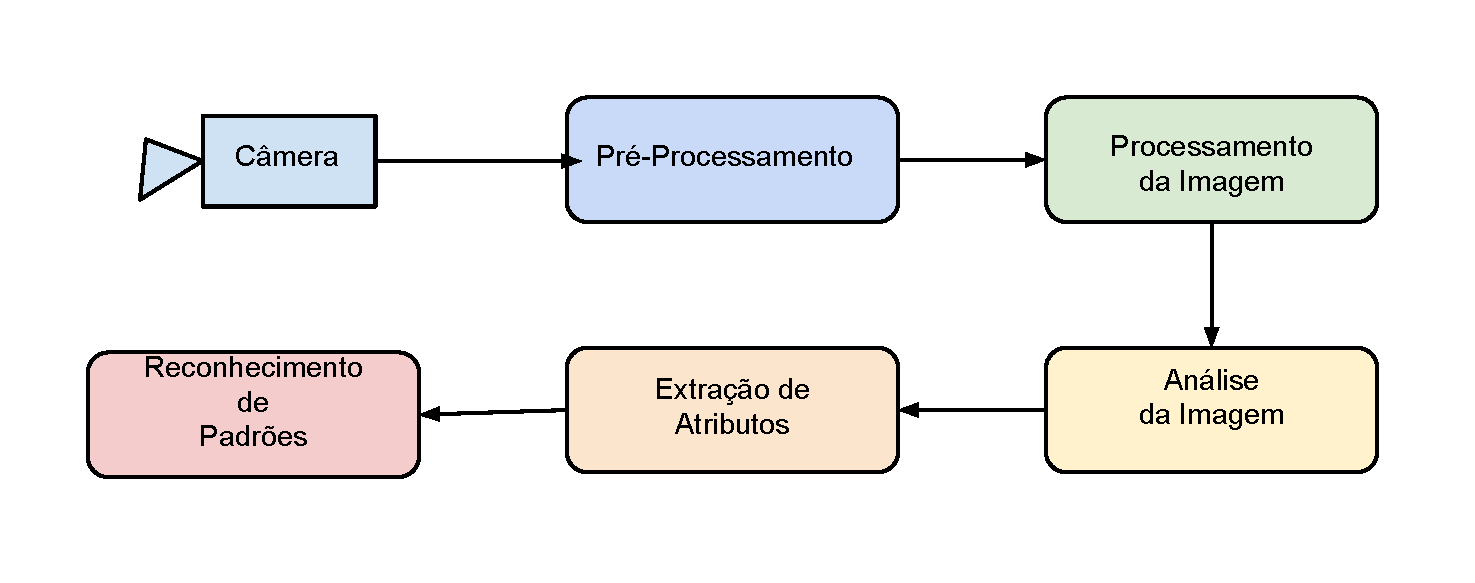
\includegraphics[width=0.9\textwidth]{Figures/ProcessosVC}
		\end{center}
		
	\end{figure}
	
\end{frame}


%%%%%%%%%%%%%%%%%%%%%%%%%%%%%%%%%%%%%%%%%%%%%%%%%%%%%%%%%%%%%%%%%%%%%%%%%%%%%%%%%%%%%%%%%%

\begin{frame}
\frametitle{Visão Computacional}

	\begin{figure}[!h]
		\begin{center}
			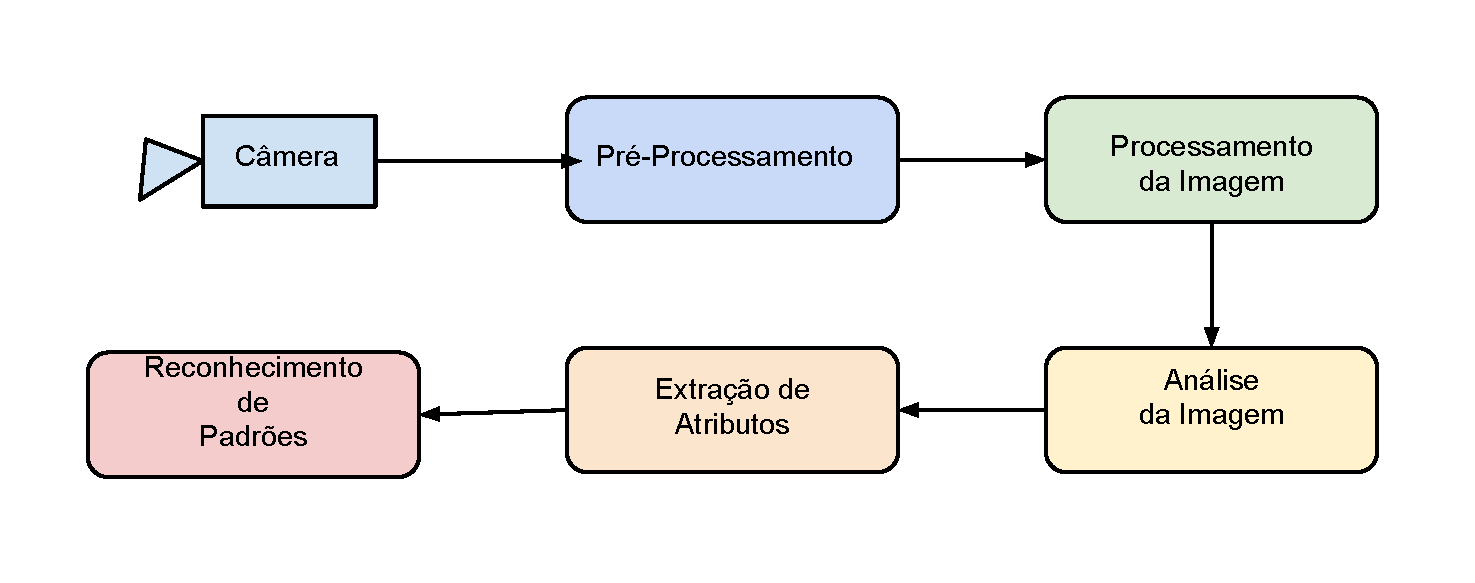
\includegraphics[width=0.9\textwidth]{Figures/ProcessosVC}
		\end{center}
		
	\end{figure}
	
\end{frame}


%%%%%%%%%%%%%%%%%%%%%%%%%%%%%%%%%%%%%%%%%%%%%%%%%%%%%%%%%%%%%%%%%%%%%%%%%%%%%%%%%%%%%%%%%%

\begin{frame}
\frametitle{Captura da Imagem}

	\begin{figure}[!h]
		\begin{center}
			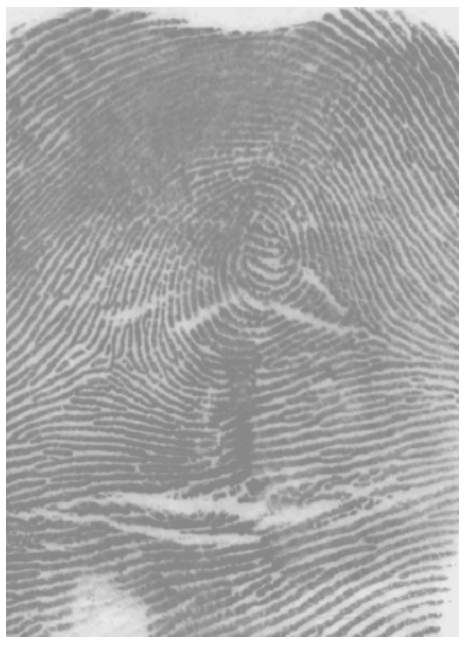
\includegraphics[width=0.5\textwidth]{Figures/digital}
		\end{center}
		
	\end{figure}
	
\end{frame}


%%%%%%%%%%%%%%%%%%%%%%%%%%%%%%%%%%%%%%%%%%%%%%%%%%%%%%%%%%%%%%%%%%%%%%%%%%%%%%%%%%%%%%%%%%

\begin{frame}
\frametitle{Pré Processamento}

	\begin{figure}[!h]
		\begin{center}
			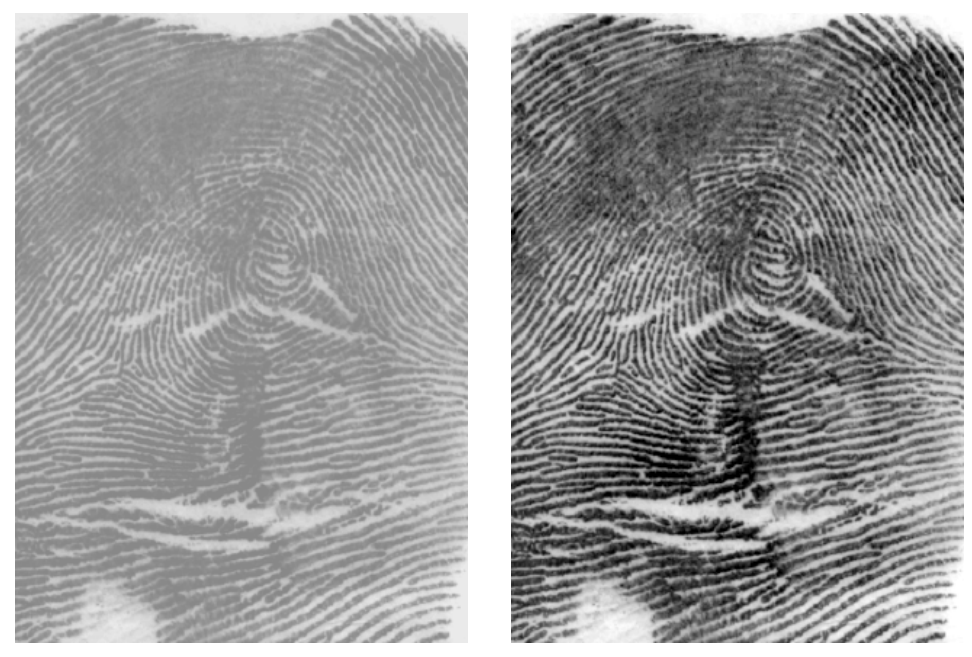
\includegraphics[width=0.9\textwidth]{Figures/prepros}
		\end{center}
		
	\end{figure}
	
\end{frame}


%%%%%%%%%%%%%%%%%%%%%%%%%%%%%%%%%%%%%%%%%%%%%%%%%%%%%%%%%%%%%%%%%%%%%%%%%%%%%%%%%%%%%%%%%%

\begin{frame}
\frametitle{Processamento}

	\begin{figure}[!h]
		\begin{center}
			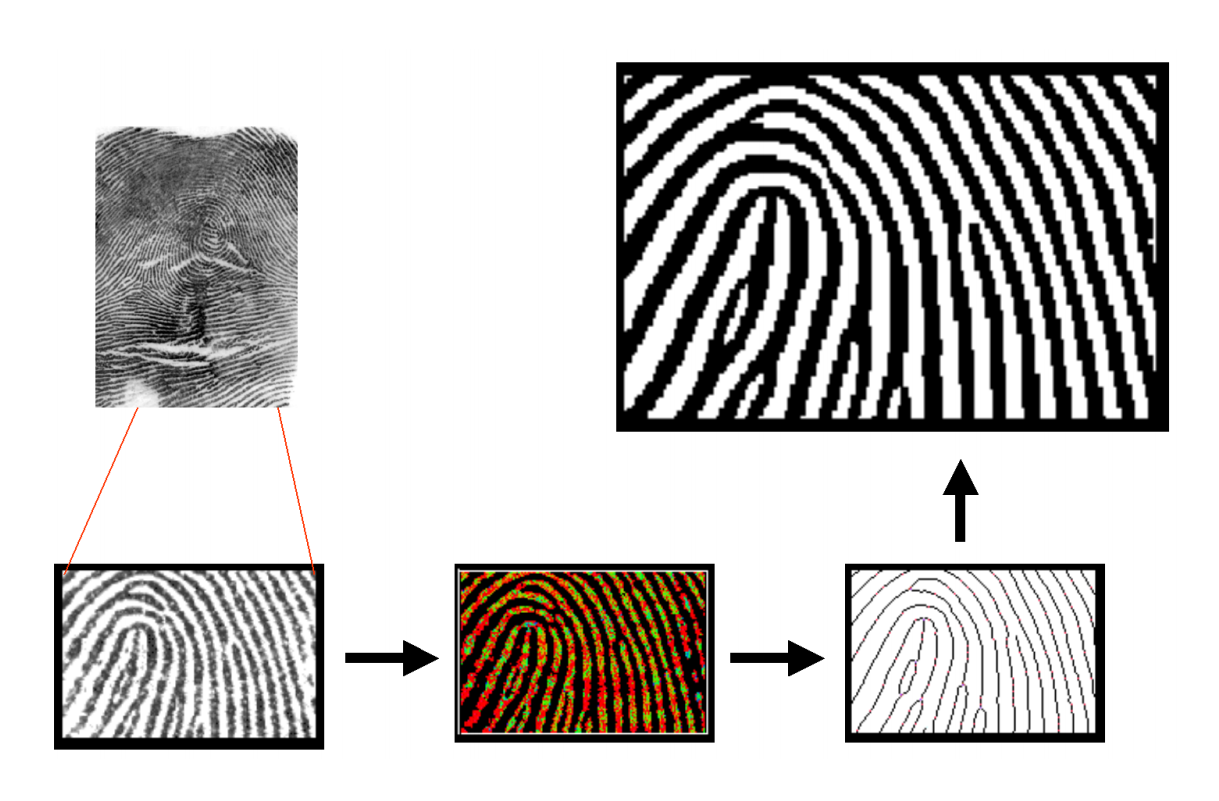
\includegraphics[width=0.9\textwidth]{Figures/process}
		\end{center}
		
	\end{figure}
	
\end{frame}

%%%%%%%%%%%%%%%%%%%%%%%%%%%%%%%%%%%%%%%%%%%%%%%%%%%%%%%%%%%%%%%%%%%%%%%%%%%%%%%%%%%%%%%%%%

\begin{frame}
\frametitle{Análise}
		
		\begin{itemize}
			\item Encontra-se todas as bifurcações.
			\item Encontra-se todas as terminações.
		\end{itemize}

	\begin{figure}[!h]
		\begin{center}
			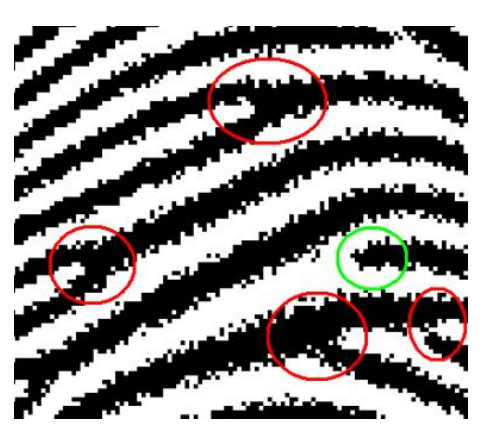
\includegraphics[width=0.5\textwidth]{Figures/features}
		\end{center}
		
	\end{figure}
	
\end{frame}

%%%%%%%%%%%%%%%%%%%%%%%%%%%%%%%%%%%%%%%%%%%%%%%%%%%%%%%%%%%%%%%%%%%%%%%%%%%%%%%%%%%%%%%%%%

\begin{frame}
\frametitle{Análise}
		
		\begin{itemize}
			\item Encontra-se todas as orientações das bifurcações.
			\item Encontra-se todas as orientações das terminações.
		\end{itemize}

	\begin{figure}[!h]
		\begin{center}
			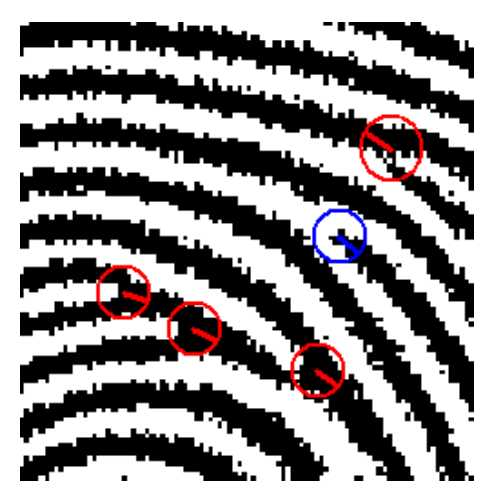
\includegraphics[width=0.5\textwidth]{Figures/orientacoes}
		\end{center}
		
	\end{figure}
	
\end{frame}

%%%%%%%%%%%%%%%%%%%%%%%%%%%%%%%%%%%%%%%%%%%%%%%%%%%%%%%%%%%%%%%%%%%%%%%%%%%%%%%%%%%%%%%%%%

\begin{frame}
\frametitle{Extração de Características}
		
		\begin{itemize}
			\item Semelhanças de triângulos.
			\item Marcar as marcações três a três.
		\end{itemize}

	\begin{figure}[!h]
		\begin{center}
			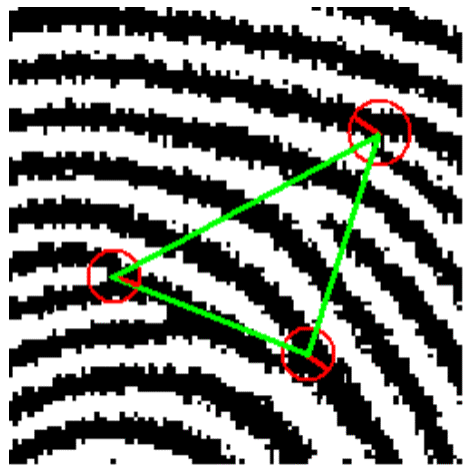
\includegraphics[width=0.5\textwidth]{Figures/semelhancas}
		\end{center}
		
	\end{figure}
	
\end{frame}

%%%%%%%%%%%%%%%%%%%%%%%%%%%%%%%%%%%%%%%%%%%%%%%%%%%%%%%%%%%%%%%%%%%%%%%%%%%%%%%%%%%%%%%%%%
\begin{frame}
\frametitle{Reconhecimento de Padrões}

	\begin{figure}[!h]
		\begin{center}
			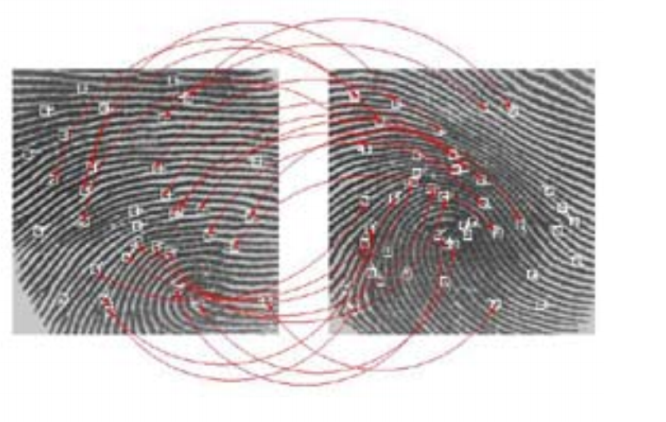
\includegraphics[width=0.8\textwidth]{Figures/reconhecimento}
		\end{center}
		
	\end{figure}
	
\end{frame}
%----------------------------------------------------------------------------------------

\end{document} 